%\documentclass[dvipdfmx,xcolor={svgnames},17pt]{beamer}
\documentclass[dvipdfmx,xcolor={svgnames}]{beamer}


\usepackage{pxrubrica}
\usepackage{color}
\usepackage{tikz}
\usepackage{pgfplots}
\usepackage{amsmath}
\usepackage{amsfonts}
\usepackage{ifthen}

\usetikzlibrary{calc}
\pgfmathsetseed{20}

\usetheme{Copenhagen}
\usecolortheme{whale}

\setbeamertemplate{caption}[numbered]
\setbeamertemplate{footline}[frame number]

\renewcommand{\figurename}{図}
\renewcommand{\tablename}{表}

\pgfplotsset{
  integral axis/.style={
        axis lines=middle,
        enlarge y limits=upper,
        axis equal image, width=12cm,
        xlabel=$x$, ylabel=$y$,
        ytick=\empty,
        xticklabel style={font=\small, text height=1.5ex, anchor=north},
        samples=100
        },
        integral/.style={
            domain=2:10,
            samples=9
            },
            integral fill/.style={
            integral,
            draw=none, fill=#1,
            on layer=axis background
            },
            integral fill/.default=cyan!10,
            integral line/.style={
            integral,
            very thick,
            draw=#1
            },
            integral line/.default=black
}

\def\vector#1{\mbox{\boldmath $#1$}}

\renewcommand{\kanjifamilydefault}{\gtdefault} % 日本語書体をゴシック体に
\renewcommand{\familydefault}{\sfdefault} % 欧文書体をHelveticaに

\title{数値解析が{\rubysizeratio{0.35}\jruby{乱数}{み|だ}}れる}
\author{13024156 藤原 渓亮}

\begin{document}

  \maketitle

  \begin{frame}{今日やること}
    \note{今日は乱数で定積分を解くモンテカルロ積分についてお話します.更に
    モンテカルロ積分に使う乱数の性能を上げた準乱数についてもお話します.
    }
    乱数で定積分を解く.\\
    準乱数で定積分を解く.
  \end{frame}

  \begin{frame}{数値積分とは}
    \note{私達が定積分を解く時は不定積分を解いてから上端と下端の値を原始関数に代入して
    解きますが,それは計算機には不可能です.数値積分とは定積分を特定の範囲における面積を表している
    と見てその面積の近似を求めることで定積分を求める方法です.}
    定積分を解析的にではなく数値的に解く
    \begin{block}{普通の積分}
      定積分 $\rightarrow$ 不定積分 $\rightarrow$ 解
    \end{block}
    \begin{block}{数値積分}
      定積分 $\rightarrow$ アルゴリズム $\rightarrow$ 近似解
    \end{block}
  \end{frame}

  \begin{frame}{数値積分の例}
    \note{数値積分の代表例として区分求積法があります.これは関数と積分範囲で囲まれた部分を
    数式で表せる図形に細かくしていきそれらの和で近似するという数値積分法です.区分求積法の
    アルゴリズムとしては以下のものがあります.}
    区分求積法
    \begin{itemize}
      \item 台形公式
      \item シンプソンの公式
      \item シンプソンの3/8公式
    \end{itemize}
  \end{frame}

  \begin{frame}{区分求積法}
    \note{区分求積法の中でも理解しやすいのが台形公式です.台形公式はその名の通り,囲まれている部分を
    台形に分割して分割した台形の面積の和を定積分の近似解とするアルゴリズムです.}
    連続値 $\rightarrow$ 離散値 \\
    ex. 台形公式
    \begin{equation*}
      \int^a_b f(x) dx \fallingdotseq \sum_{k=0}^{n-1} \frac{\{f(x_{k+1}) + f(x_k)\}(x_{k+1}-x_k)}{2}
    \end{equation*}
  \end{frame}

  \begin{frame}{区分求積法}
    \note{区分求積法を分かりやすく図にしたものです.
    下端の値がaで上端の値がbです.このように積分の区間を細かく分割して台形と見なしてそれらの面積の和を
    取ることで関数と積分範囲で囲まれている部分の面積に近似できているのがわかると思います.}
    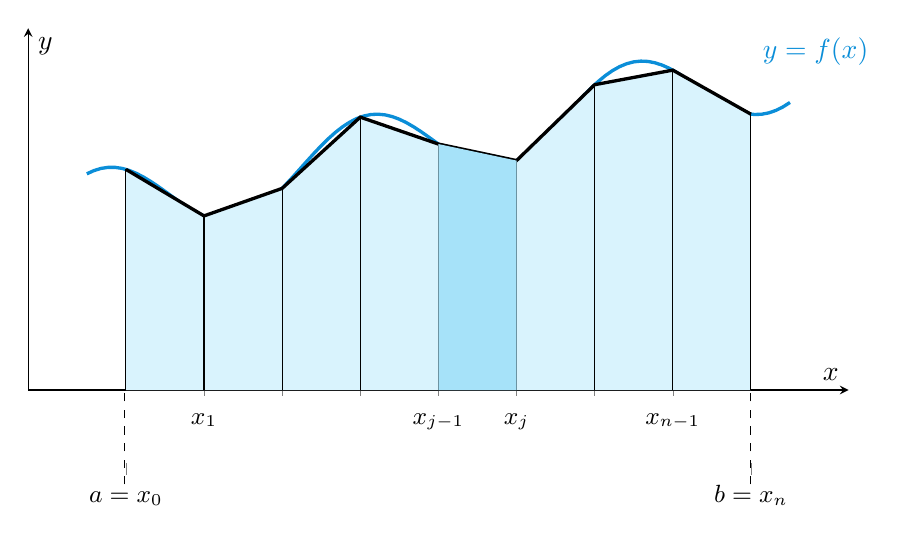
\begin{tikzpicture}[declare function={f=x/5-cos(deg(x*1.85))/2+2;}]
      \begin{axis}[
        integral axis,
        ymin=0,
        xmin=0.75, xmax=11.25,
        domain=1.5:10.5,
        xtick={3,...,9},
        extra x ticks={2,10},
        extra x tick labels={$a=x_0$, $b=x_n$},
        xticklabels={$x_1$,,,$x_{j-1}$,$x_j$,,$x_{n-1}$},
        extra x tick style={yshift=-1cm, anchor=south}
        ]

        % The function
        \addplot [very thick, cyan!75!blue] {f};

        % The filled area under the fallingdotseqimate integral
        \addplot [integral fill=cyan!15] {f} \closedcycle;

        % The fallingdotseqimate integral
        \addplot [integral line=black] {f};

        % The vertical lines between the segments
        \addplot [integral, ycomb] {f};

        % The highlighted segment
        \addplot [integral fill=cyan!35, domain=6:7, samples=2] {f} \closedcycle;
      \end{axis}
      \draw[dashed] (1.2275,-1.2) -- (1.2275,0);
      \draw[dashed] (9.175,-1.2) -- (9.175,0);
      \draw[cyan!75!blue] (10,4) node [above] {$y=f(x)$};
    \end{tikzpicture}
  \end{frame}

  \begin{frame}
    \note{というわけで区分求積法は計算機でも計算することが可能です.それではモンテカルロ積分の
    需要はあるのでしょうか.実は1次積分の時は区分求積法の法がよいのですが重積分のような高次元の
    関数に対する積分は計算量的に差がでてきます.}
    区分求積法なら計算機で計算できる. \\
    モンテカルロ積分の存在意義は? \\
    \pause
    $\rightarrow$ 重積分
    \begin{equation*}
      \idotsint f(x_1,x_2,\ldots x_L) dx_1dx_2\cdots dx_L
    \end{equation*}
  \end{frame}

  \begin{frame}{計算量}
    \note{区分求積法の計算量はL重積分に対しオーダはNのL乗となります.それに対し
    モンテカルロ法の計算量はオーダNLになります.}
    \begin{block}{区分求積法}
      L重積分をN個に分割する,\\ 計算量は \\
      $\rightarrow O(N^L)$
    \end{block}
    \begin{block}{モンテカルロ法}
      L重積分に対しN個の点をプロット,\\ 計算量は \\
      $\rightarrow O(NL)$
    \end{block}
  \end{frame}

  \begin{frame}{乱数(列)とは}
    \note{次にモンテカルロ法で必須な乱数についてお話します.乱数は
    主に次のような条件を満たす数値または数列のことを言います.}
    出力が一意的ではない数字のこと,法則性がない数列のこと
    \begin{itemize}
      \item 予測不可能性
      \item 一様性
      \item 非周期性
      \item 非再現性
    \end{itemize}
  \end{frame}

  \begin{frame}{予測不可能性}
    \note{予測不可能性とは今まで出力された乱数から次に出てくる乱数を予測することは
    不可能であるということです.サイコロを振って出た目から次に振った目を予測することは
    不可能であることと一緒です.一般的には独立性ともいいます.}
    $x_0,x_1\ldots x_n$から$x_{n+1}$は予測できない.
  \end{frame}

    \begin{frame}{一様性}
      \note{一様性とは乱数生成器が生成できる値であるならばどの値も出力される確率は
      一緒で全通りの値分の一となります.}
      \begin{equation*}
        P(x=X) = \frac{1}{\beta - \alpha} (\alpha \leq x \leq \beta)
      \end{equation*}
      \begin{figure}[htbp]
        \centering
        \includegraphics[scale=0.3]{MTrand.png}
      \end{figure}
    \end{frame}

    \begin{frame}{非周期性}
      \note{非周期性はいくら乱数を出力しても過去に出た乱数のパターンは現れないということです.
      乱数列は無限に続きループしないということです.}
      同じパターンの数列が現れない.
    \end{frame}

    \begin{frame}{非再現性}
      \note{非再現性とは乱数列は同じ条件を揃えて同じ乱数列を出力することができないということです.}
      初期値が同じでも異なる数列が出現する.
    \end{frame}

    \begin{frame}{疑似乱数}
      \note{疑似乱数は計算機で出力する乱数のように見える数列です.}
      厳密には決定的であるが乱数列のように見える数列
      \begin{itemize}
        \item 予測不可能性 $\rightarrow$ △
        \item 一様性 $\rightarrow$ △
        \item 非周期性 $\rightarrow$ x
        \item 非再現性 $\rightarrow$ x
      \end{itemize}
    \end{frame}

    \begin{frame}{予測不可能性 $\rightarrow$ △}
      \note{出力は決定的なので予測をすることが可能です.特定の疑似乱数生成器から出力された
      乱数を元に逆問題的に疑似乱数生成器の式や定数を求めることが可能です.しかし,暗号化などに
      使われる疑似乱数生成器は一方向関数と呼ばれ逆問題的に式を求めることは計算量的に不可能とされています.}
      ex) 線形合同法
      \begin{align*}
        \vector{x} &= \{x_0,x_1,\ldots x_n, \ldots\} \\
        x_{n+1} &= (Ax_n + B) \bmod M (A,B,M \in \mathbb{Z})
      \end{align*}
      $x_0,A,B,M$が分かれば予測可能
    \end{frame}

      \begin{frame}{一様性 $\rightarrow$ △}
        \note{現在使われているメルセンヌツイスターという疑似乱数アルゴリズムはある程度は均等に分布しますが,
        線形合同法というアルゴリズムは3次元ベクトルの乱数を出力した時に偏りがあることが知られています.線形合同法は
        元々偶数と奇数が交互に出力される時点で一様性が失われています.}
        \begin{figure}[htbp]
          \includegraphics[scale=0.3]{lcm.jpg}
        \end{figure}
        粗悪なアルゴリズム $\rightarrow$ 高次元にて偏る.
      \end{frame}

      \begin{frame}{非周期性 $\rightarrow$ x}
        \note{現在の計算機には限度がありどんなに優れたアルゴリズムでも周期は存在します.}
        \begin{block}{線形合同法}
          $2^{32} - 1$
        \end{block}
        \begin{block}{$n$ビット線形帰還シフトレジスタ}
          $2^n - 1$
        \end{block}
        \begin{block}{メルセンヌ・ツイスタ}
          $2^{19937} - 1$
        \end{block}
        必ず,周期はある
      \end{frame}

      \begin{frame}{非再現性 $\rightarrow$ x}
        \note{大抵の疑似乱数アルゴリズムは何らかの漸化式で表される為,同じ初期値を与えると
        同じ出力をします.}
        計算機の出力は決定的
      \end{frame}

      \begin{frame}{モンテカルロ積分}
        \note{モンテカルロ積分はその名の通り定積分をモンテカルロ法で解くことです.}
        定積分をモンテカルロ法で解くこと
      \end{frame}

      \begin{frame}{モンテカルロ法とは}
        \note{それでは,モンテカルロ法とは何か.まず,モンテカルロとはモナコ公国にあるモンテカルロ地区という
        地名です.国営カジノがあり,ギャンブルで有名です.}
        \begin{figure}
          \centering
          \includegraphics[scale=0.15]{monte.jpg}
          \caption{モナコ公国モンテカルロ地区}
          \label{fig:two}
        \end{figure}
      \end{frame}

      \begin{frame}{モンテカルロ法とは}
        \note{そして,モンテカルロ法とは乱数を用いて数値計算を行う乱択アルゴリズムの一つです.
        乱択アルゴリズムはアルゴリズムに確率性を持たせ決定性アルゴリズムよりも確率的に早く処理を終わらせる
        アルゴリズムです.乱択アルゴリズムは以下の2つに大別されます.これからやっていくモンテカルロ法は
        処理の結果が一定の確率で間違っていても構わないとするアルゴリズムで,ラスベガス法とは
        乱数を用いて場合によっては速くなるが速さよりも正当性を重視するアルゴリズムです.}
        乱数を用いて数値計算を行う方法 \\
        乱択アルゴリズム \\
        \begin{itemize}
          \item モンテカルロ法 \visible<2,2>{$\rightarrow$ 一定の確率で誤る}
          \item ラスベガス法 \visible<2,2>{$\rightarrow$ いつでも正答する}
        \end{itemize}
      \end{frame}

      \begin{frame}{例題}
        \note{それでは今回モンテカルロ法で以下の積分を使って円周率の近似を求めます.
        まずは手計算でやるとどうなるでしょうか.}
        \begin{minipage}{0.4\textwidth}
          \begin{equation*}
            \int^1_0 \sqrt{1 - x^2}dx
          \end{equation*}
          を解け
        \end{minipage}
        \begin{minipage}{0.5\textwidth}
          \centering
          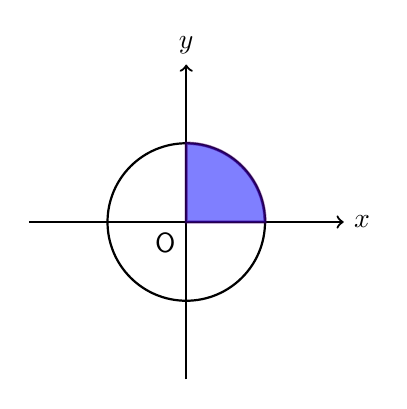
\begin{tikzpicture}[domain=0:8, samples=100, very thick] % 定義域、点の数、線幅
            \draw (0,0) node[below left]{O}; % 原点、0でも、above, below, left, rightで位置指定
            % 位置指定はanchor=north, south, east, westでも可能
            \draw[thick, ->] (-2,0)--(2,0) node[right] {$x$}; % x軸、[->]で矢印、他に[-stealth]等
            \draw[thick, ->] (0,-2)--(0,2) node[above] {$y$}; % y軸

            %\draw plot[domain=-1:1](\x, {sqrt(1-\x^2)}) node[above]{$f(x)=x^2-3x+2$}; % atでnodeの位置指定
            %\draw plot[domain=-1:1](\x, {-sqrt(1-\x^2)}) node[above]{$f(x)=x^2-3x+2$}; % atでnodeの位置指定
            \draw [thick] (0,0) circle (1);
            \filldraw [fill=blue, opacity=.5, draw=Indigo] (1,0)  arc (0:90:1) --(0,0)--cycle;
          \end{tikzpicture}
        \end{minipage}

      \end{frame}

      \begin{frame}
        \note{これは置換積分です.}
        \begin{align*}
          &\int^1_0 \sqrt{1 - x^2}dx \\
          \intertext{$x = \cos\theta$と置く}
          &= \int^{1}_0 \sqrt{1 - \cos^2\theta} dx \\
          \intertext{$dx = -\sin\theta d\theta$より}
          &= \int^{\frac{\pi}{2}}_0 \sqrt{1 - \cos^2\theta}(-\sin\theta) d\theta
        \end{align*}
      \end{frame}

      \begin{frame}
        \note{半角の公式を使って積分できる形に直します.答えはよんぶんのパイになります.
        四倍したら円周率になります.}
        \begin{align*}
          &= -\int^{\frac{\pi}{2}}_0 \sin^2\theta d\theta \\
          \intertext{半角の公式より}
          &= -\frac{1}{2}\int^{\frac{\pi}{2}}_0 1 - 2\cos2\theta d\theta \\
          &= -\frac{1}{2}[\theta + \sin2\theta]^{\frac{\pi}{2}}_0 = \frac{\pi}{4}
        \end{align*}
      \end{frame}

      \begin{frame}{モンテカルロ積分}
        \note{この図は今計算した積分を図にしたものです.モンテカルロ法は計算したい部分を覆うように
        正方形を描いて考えます.第一段階としてこの正方形の中にランダムに点をプロットしていきます.
        そして,プロットした点が積分範囲内なのかどうかを判定して範囲内にある点をカウントします.
        最終的に範囲内にある点の数と全体の点の数の比は求めたい面積と正方形の面積の比を一緒とみなす
        ことで求めたい面積もとい定積分の近似解を得るというアルゴリズムです.}
        \begin{tikzpicture}[declare function = {Circle(\x)= sqrt(5-\x)*sqrt(5+\x);}]
          \draw [ultra thick] (0,0) rectangle (5,5);
          \draw [] (0,5)  arc (180:120:0.5);
          \draw [] (5,5)  arc (0:45:0.5);
          \draw (2.5,5.5) node {2};
          \draw [thick] (5,0)  arc (0:90:5) --(0,0)--cycle;
          \foreach \i in {1,...,10}
          {
            \foreach \j in {1,...,100}
            {
             \pgfmathsetmacro\myX{random(0,4) + random(0,1000)/1000}%
             \pgfmathsetmacro\myY{random(0,4) + random(0,1000)/1000}%
             \pgfmathsetmacro{\rndcolor}{ Circle(\myX)<\myY ? "red" : "blue" }
             \filldraw[fill=\rndcolor] (\myX, \myY) circle [radius=0.05];
            }

            \pause

          }
          \draw (9,5) node {青い点数 = $m$};
          \draw (9,4) node {赤い点数 = $n$};
          \draw (9,3) node {全体的な面積 = $4$};
          \draw (9,2) node {求めたい面積 = $x$};
          \draw (9,1) node {$m : n \fallingdotseq x : 4$};
        \end{tikzpicture}
      \end{frame}

      \begin{frame}{演習1}
        \note{ex.cppにあるmontecarlo関数を完成させてください.}
        モンテカルロ積分のプログラムを \\
        完成させよ.

      \end{frame}

      \begin{frame}{休憩}
        続きは午後から
      \end{frame}

      \begin{frame}{準乱数}
        \note{午前はモンテカルロ法を使って円周率の近似解を求めました.それでは次に準乱数を使った
        準モンテカルロ法についてやっていきます.準乱数はランダム性がなくなってその代わりに一様性を
        高めた乱数です.具体的に言えば疑似乱数は少ないプロット数では一様になりづらいのに対し
        準乱数は少ないプロット数で一様になるという特長があります.}
        \begin{tikzpicture}
          \draw (0,0) node {ランダム性};
          \draw[->,ultra thick] (0,-1) -- (0,-3);
          \draw[ultra thick] (-0.5,-4) -- (0.5,-5);
          \draw[ultra thick] (0.5,-4) -- (-0.5,-5);

          \pause

          \draw[->,ultra thick] (6,-1) -- (6,-3);

          \draw (6,0) node {一様性};
          \draw [red, thick] (6,-4.5) circle (0.7);
          \draw [red, thick] (6,-4.5) circle (0.5);
        \end{tikzpicture}
      \end{frame}

      \begin{frame}{疑似乱数と準乱数}
        \note{以下は疑似乱数と準乱数を100個ずつプロットした図です.見れば分かるように
        準乱数の方が一様に分布しています.少ないプロットで一様に分布するとモンテカルロ法によって
        求まる近似解の精度がよくなります.詳しい計算は省きますがモンテカルロ法の近似精度を10倍にするには
        疑似乱数の場合はプロット数を100倍にしなければなりませんが,準乱数の方は10倍で済みます.}
        \begin{figure}
          \begin{minipage}{0.45\hsize}
            \centering
            \includegraphics[width=\columnwidth]{mersenne.pdf}
            \caption{MT}
          \end{minipage}
          \begin{minipage}{0.45\hsize}
            \centering
            \includegraphics[width=\columnwidth]{halton.pdf}
            \caption{Halton}
          \end{minipage}
        \end{figure}
      \end{frame}

      \begin{frame}{van der corput列}
        \note{それでは準乱数の具体的な計算方法についてお話します.準乱数の一種にファンデルコルプト列というものがあります.
        ファンデルコルプト列は以下の逆基底関数で求まります.bは基底と呼び任意の素数を取ります.nは任意の整数です.}
        基底$b$の逆基底関数$\phi_b$で定義される.
        \begin{align*}
          \phi_b(n) = \sum_{ i\leq 0} d_ib^{-i-1} = \sum_{ i\leq 0} \frac{d_i}{b^{i+1}}\\
          \{\phi_b(0), \phi_b(1), \phi_b(2), \ldots ,\phi_b(n)\}
        \end{align*}
      \end{frame}

      \begin{frame}
        \note{dはnをb進表記した時のそれぞれの桁になります.}
        $d_i$は$n$を$b$進表記した時の$i$ビット目.
        \begin{align*}
          10_{(10)} &=
          {\color<1,1>{red}{1}}
          {\color<2,2>{red}{0}}
          {\color<3,3>{red}{1}}
          {\color<4,4>{red}{0}}_{(2)} \\
          \color<4,4>{red}d_0 &\color<4,4>{red}= 0 \\
          \color<3,3>{red}d_1 &\color<3,3>{red}= 1 \\
          \color<2,2>{red}d_2 &\color<2,2>{red}= 0 \\
          \color<1,1>{red}d_3 &\color<1,1>{red}= 1
        \end{align*}
      \end{frame}

      \begin{frame}
        \note{例としてb=2,n=10の時の逆基底関数を見ていきます.10を2進数表記した時は
        1010になります.これらがそれぞれdの値になります.これらが求まれば後は元の式に代入するだけ
        です.}
        \begin{align*}
          \phi_2(10) &= 1\times 2^{-3-1} + 0\times 2^{-2-1}  \\
          &+ 1\times 2^{-1-1} + 0\times 2^{-0-1} \\
          &= \frac{1}{2^4} + \frac{1}{2^2} \\
          &= \frac{3}{8}
        \end{align*}
      \end{frame}

      \begin{frame}{Halton列}
        \note{そして,今回の準モンテカルロ法に使うHalton列を紹介します.Halton列はファンデルコルプト列を
        高次元にしたものです.積分値は2次元以上になるのでHalton列を用います.}
        van der corput列を高次元にしたもの
        \begin{align*}
          X_n = \{\phi_{b1}(n), \phi_{b2}(n), \phi_{b3}(n), \ldots ,\phi_{b4}(n)\}
          \intertext{ただし,$b1,b2,\ldots ,bn$は全て素数}
        \end{align*}
      \end{frame}

      \begin{frame}{演習2}
        \note{まずはファンデルコルプト列を実装します.ex.cppの中にある van der corput関数を完成させてください.}
        van der corput列を実装せよ.\\
        \begin{block}{ヒント}
            $vdc(b,n,i) = \frac{(n\bmod b)}{b^{i+1}} + vdc(b, \frac{n}{b}, i+1)$
        \end{block}
      \end{frame}

      \begin{frame}{演習3}
        \note{van der corput列が完成したら次はquasimontecarlo関数を完成させてください.}
        準モンテカルロ法を完成させよ.\\
      \end{frame}

      \begin{frame}{演習4}
        \note{以下の積分を求めてください.手計算でできるのであればやってみても構いません.}
        以下の(近似)解を求めよ.
        \begin{equation*}
          \int_0^3 \!\!\! \int_0^2 \!\!\! \int_0^1  x^2y^2z^2exp(-(x^2+y^2+z^2)) dxdydz
        \end{equation*}
        \pause
        $\fallingdotseq 0.0354754$

      \end{frame}
\end{document}
